\documentclass[svgnames,12pt,aspectratio=149]{beamer}
\mode<presentation>%
{
  \usetheme{Boadilla}
  \setbeamercovered{dynamic}
}
\usepackage[english,spanish]{babel}
\usepackage[utf8]{inputenc}
\usepackage[T1]{fontenc}
\usepackage{sty/BeamerLille}
\usepackage{float}
\usepackage{caption}
\usepackage{subfigure} 
\usepackage{quantikz}
\usepackage{graphicx}
\usepackage{dsfont}
\graphicspath{ {./images/} }
\usepackage{tikz}
\renewcommand\qedsymbol{$\blacksquare$}
\newcommand{\ra}{\rangle}
\newcommand{\la}{\langle}
\newcommand{\rala}{\rangle\langle}
\newcommand{\tr}{{\rm Tr}}
\newcommand{\E}{\mathcal{E}}
\newcommand{\tensor}{\otimes}
\newcommand{\prodtensor}{\bigotimes_{i=1}^{N}}
\newcommand{\fuzzy}[1]{\mathcal{F}\left(#1\right)}
\newcommand{\fuzzydagger}[1]{\mathcal{F}^{\dagger}\left(#1\right)}
\newcommand{\permut}[2]{\Pi_{#1}#2\Pi_{#1}^{\dagger}}
\newcommand{\permutdagger}[2]{\Pi_{#1}^{\dagger}#2\Pi_{#1}}


\usepackage{amssymb,amsfonts}


\title{Mediciones difusas en sistemas cuánticos\\\hspace{0.7cm}para N partículas}
\subtitle{}
\author[Rubí Ramírez] % (optional)
{Rubí Ramírez Milián}
\institute[ECFM]{
Escuela de Ciencias Físicas y Matemática\\
Universidad de San Carlos\\
\textit{Asesorado por: \\ 
Dr.\@ Carlos Pineda (IF-UNAM)}\\
Ing. Rodolfo Samayoa (ECFM-USAC)
}
\date{14 de agosto de 2024}
\AtBeginSection[]
{
 \begin{frame}
    \frametitle{Contenidos}
	\tableofcontents[currentsection]
  \end{frame}
}

\begin{document}

\begin{frame}[plain]
  \titlepage{}
\end{frame}

\begin{frame}{Agradecimientos}
     \begin{itemize}
  \item A mi familia
  \item A mis asesores
  \item A mis amigos y amigas
  \end{itemize}
\end{frame}


\section{Introducción}

\begin{frame}
  \frametitle{Motivación}
 En la práctica  las mediciones que se realizan son imperfectas es por ello que es necesario un formalismo más extenso para poder proporcionar una descripción completa de las mediciones no ideales. 

 Para describir apropiadamente las mediciones difusas es necesario un mapeo de probabilidad de obtener las posibles salidas y el estado posterior a la medición.


\end{frame}

\begin{frame}
  \frametitle{Introducción}
\begin{itemize}
  \item  Se inicia con un marco conceptual que contiene las herramientas más básicas  en la descripción de mediciones en sistemas cuánticos.
  \item Se presenta el problema de las mediciones difusas de manera concreta.
  \item Se tratan los resultados obtenidos para sistemas de dos partículas para posteriormente generalizarlos.
\end{itemize}

\end{frame}






\section{Revisión de literatura}
\begin{frame}
 \frametitle{Operador de densidad}
 
 \begin{block}{}
  El operador de densidad que corresponde al ensamble de estados puros $ \{p_j,|\psi_j\rangle\}$ es tal que \[\rho=\sum_j p_j |\psi_j\rangle\langle\psi_j|.\]

 \end{block}
 

\end{frame}

\begin{frame}
\frametitle{Medidas POVM}
    \begin{block}{}
      Una medida POVM (positive operator-valued measure) 
Las medidas POVM son  un conjunto $\{E_{m}\}$ de operadores llamados <<efectos>> que satisfacen las siguientes condiciones:
\begin{enumerate}
    \item Positividad: $\langle \psi |E_m|\psi \rangle \ge 0 $ para cualquier vector $|\psi\rangle$.
    \item Hermiticidad: $E_m=E_{m}^\dagger$.
    \item  Completitud: $\sum_m E_m =\mathds{1}$.
\end{enumerate}
    \end{block}
  Brindan el mapeo de probabilidades \begin{equation*}\begin{split}
      E:S\times \mathcal{B(H)}\longrightarrow [0,1]\\
      E(m,\rho)=\text{Tr}(E_m\rho).
  \end{split}\end{equation*}


\end{frame}

\begin{frame}{Operadores de Kraus}
  Por otra parte los operadores de Kraus son un conjunto de operadores $\{K_i\} $ que representan una operación cuántica en forma de suma \begin{equation*}
    \E(\rho)=\sum_i K_i\rho K_i^\dagger \end{equation*}
\end{frame}







\section{Mediciones difusas}

\begin{frame}{Mediciones difusas}
Una medición difusa es un proceso no ideal en el cual, debido a ruido
del entorno o a fallos en el dispositivo de detección, se presenta la probabilidad de una
identificación errónea de las partículas del sistema.
\vspace{1cm}
\begin{figure}[H]
  \centering
 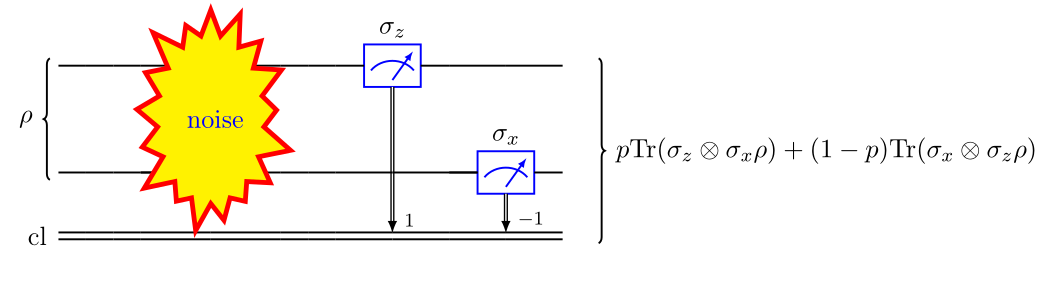
\includegraphics[width=100mm]{images/fm1.png}
  \caption*{}
\end{figure} 
\end{frame}



\begin{frame}{Valor esperado y operador difuso}

 
Para un sistema de dos partículas el valor esperado de un observable factorizable es 
\begin{equation*}\label{eq:Expected-Value-FM-2p}
    \begin{split}
      \la {A\otimes B}\ra_{\mathcal{F}_{2\text{p}}(\rho)} =&p\tr(\rho A\tensor B)+(1-p)\tr(\rho B\otimes A).\\
    \end{split}
\end{equation*}Lo que permite introducir al operador difuso que se define como \begin{equation*}\label{eq:op_F2p}
    \mathcal{F}_{2\text{p}}(\rho):=p\rho + (1-p)S_{12}\rho S_{12}^{\dagger}.
\end{equation*}
Para sistemas más grandes es 
\begin{equation*}\label{eq:expected-value-fm-general}
    \la \mathcal{O}\ra_{\fuzzy{\rho}}=\sum_{i}p_i\tr(\permut{i}{\rho}\mathcal{O}) =\tr(\fuzzy{\rho}\mathcal{O}).
\end{equation*} donde \begin{equation*}\label{eq:fuzzy-op-nparticles}
    \fuzzy{\rho}=\sum_{i}p_{i}\permut{i}{\rho}
 \end{equation*} con $\Pi_i \in \mathcal{S}$ son los operadores de permutación.

\end{frame}

\begin{frame}{Instrumentos cuánticos}
  Son un ensamble que correlaciona un sistema clásico y que contiene la salida de la medición y un sistema cuántico que contiene el estado posterior a la medición \begin{equation*}
    \begin{split}
        \mathcal{I}: \mathcal{B(H)}\rightarrow\mathcal{B(H)}_{\text{cl}}\otimes \mathcal{B(H)}_{\text{qu}},\\
    \mathcal{I}(\rho)=\sum_\alpha |\alpha\rala\alpha|\otimes \E_\alpha(\rho).
    \end{split}
\end{equation*}
\end{frame}


\section{Resultados}
\begin{frame}{POVM y operadores de Kraus para mediciones difusas en sistemas de dos partículas}
  Los efectos para una medición difusa son \[\{\mathcal{F}_{2\text{p}}(P_{a_j,b_k})\}\]los cuales proporciona el mapeo de probabilidades tal que \[   E(a_j b_k, \rho)= \tr(\mathcal{F}_{2\text{p}}({P_{a_j,b_k}})\rho).\] Es necesario descomponer estos efectos, definiendo un conjunto de operadores de Kraus de manera que se cumpla que \[\mathcal{F}_{2\text{p}}(P_{a_j,b_k})=K_{a_j,b_k}^\dagger K_{a_j,b_k}.\] Por tanto se pueden considerar los siguientes operadores \[K_{a_j,b_k}=\sqrt{\mathcal{F}_{2\text{p}}(P_{a_j,b_k}\rho)}.\]
\end{frame}



\begin{frame}{Instrumentos cuánticos para dos partículas I}
  \begin{equation*}\label{eq:fisrtinstrument2p}
    \begin{split}
        \mathcal{I}_1{(\rho)}&=\sum_{j,k}P_{a_j,b_k}\otimes P_{a_j,b_k} \mathcal{F}_{2\text{p}}(\rho) P_{a_j,b_k}\\
        &=\sum_{j,k}P_{a_j,b_k}\otimes P_{a_j,b_k} [p \bra{a_j b_k}\rho \ket{a_j,b_k}+(1-p)\bra{b_k a_j }\rho \ket {b_k a_j}],
\end{split}
\end{equation*}
\begin{figure}[H]
\centering
\subfigure[]{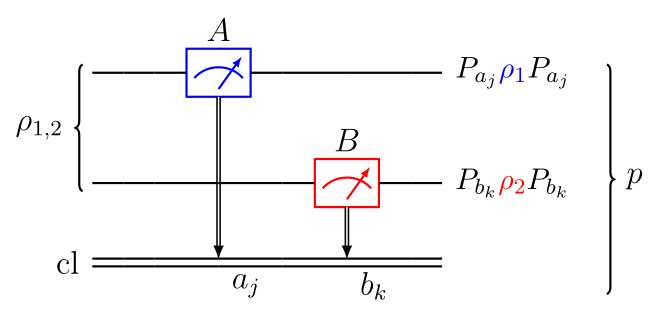
\includegraphics[width=50mm]{images/fmideaqi.png}}
\subfigure[]{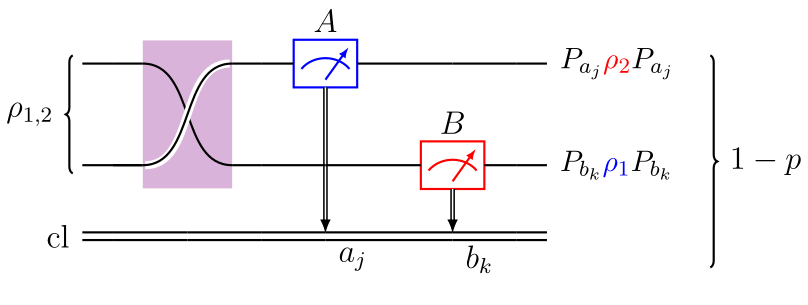
\includegraphics[width=60mm]{images/fmqi1.png}}
\caption*{}
\end{figure} 




\end{frame}

\begin{frame}{Instrumentos cuánticos para dos partículas II}
  \begin{equation*}\label{eq:second-instrument-2p}
    \begin{split}
        \mathcal{I}_2(\rho)&=\sum_{j,k}\mathcal{F}_{2\text{p}}(P_{a_j,b_k})\otimes P_{a_j,b_k} \rho P_{a_j,b_k}\\
    \end{split}
\end{equation*} 
\begin{figure}[H]
\centering
\subfigure[]{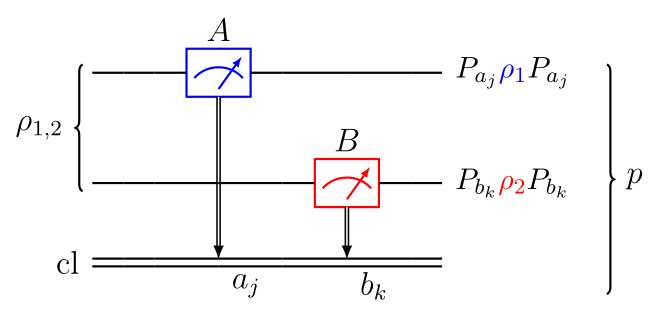
\includegraphics[width=60mm]{images/fmideaqi.png}}
\subfigure[]{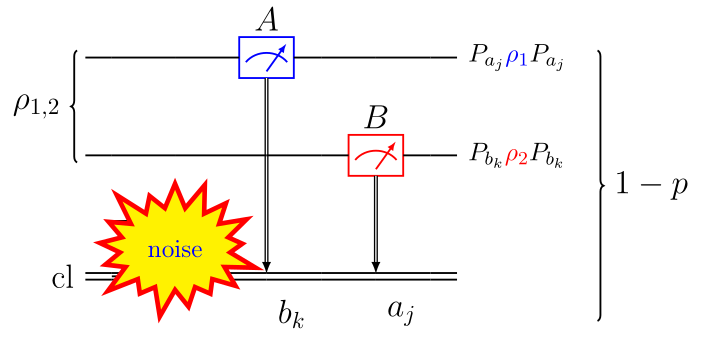
\includegraphics[width=60mm]{images/fmqi2.png}}
\caption*{}
\end{figure} 

\end{frame}

\begin{frame}{Instrumentos cuánticos para dos partículas III}
  \begin{equation*}\label{eq:quantum-instrument-3-desarrollo}
    \begin{split}
        \mathcal{I}_3(\rho)&=q\sum_{m,n}  P_{a_m,b_n}\otimes P_{a_m,b_n}\rho P_{a_m,b_n}\\
        &+(1-q)\left[\sum_{(j,k)\in K}P_{a_j,b_k} \otimes P^{K}_{a_j,b_k}\rho P^{K}_{a_j,b_k}+\sum_{(i,l) \in L}P_{a_i,b_l} \otimes  \dfrac{1}{2}P^{L}_{a_i,b_l}\rho P^L_{a_i,b_l}\right]\\
    \end{split}
\end{equation*}
\begin{figure}[H]
    \centering
\subfigure[]{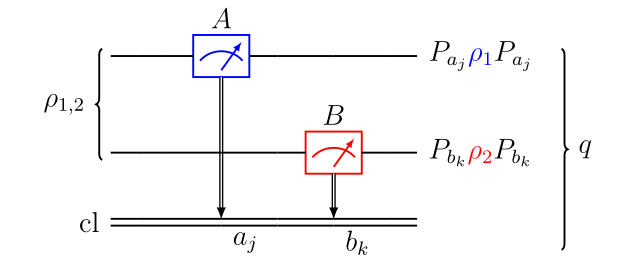
\includegraphics[width=55mm]{images/fmidealiq3.png}}
\subfigure[]{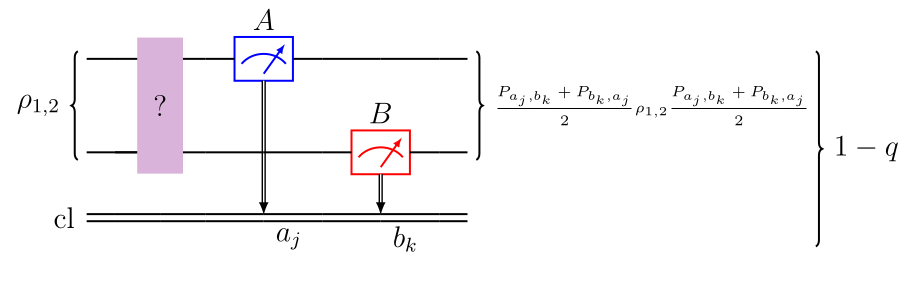
\includegraphics[width=70mm]{images/fmqi3.png}}
\caption*{} 
\end{figure} 
\end{frame}

\begin{frame}{Equivalencia}
  \begin{block}{Proposición: Equivalencia entre instrumentos I y II}
    Para todo estado inicial $\rho$, los valores esperados de las alternativas
de los instrumentos cuánticos I y II son equivalentes si y solo si \begin{equation*}\label{eq:Condicion-equivalencia1-2}
    \la a_j
b_k|B\otimes A|a_{j'}b_{k'}\ra=0, \forall j,k\ne j',k'.
\end{equation*}
\end{block}

%\begin{proposition}
 %   Si se satisface la condición  \[\la a_j b_k|B\otimes A|a_{j'}b_{k'}\ra=0, \forall j,k\ne j',k', \]  entonces $[A\otimes B,B \otimes A]=0$  
%end{proposition}


\begin{block}{Proposición: Equivalencia entre instrumentos I y III}
    Para todo estado inicial $\rho$, los valores esperados de las alternativas
de instrumentos cuánticos I y III son equivalentes si y solo si
$p=\dfrac{1+q}{2}$.
\end{block}
\end{frame}


\begin{frame}{Generalización}
  La clave para lograr los efectos de manera correcta es también emplear el valor esperado de una medición difusa. Los efectos pueden escribirse como
  \begin{equation*}
      {\{E_{\lambda_i}\}}_{\lambda_i \in \Lambda}={\left\{\sum_{j} p_{j} \permutdagger{j}{P_{\lambda_i}}\right\}}_{\lambda_i \in \Lambda},
  \end{equation*}  
  Los respectivos operadores de Kraus 
  \begin{equation*}
     K_{\lambda_i}=\sqrt{\sum_{j} p_j \permutdagger{j}{P_{\lambda_i} }},
  \end{equation*} 
  esto se puede realizar debido a la positividad de los efectos.
\end{frame}


\begin{frame}{Generalización de Instrumentos}
  La generalización de los primeros dos instrumentos es fácilmente realizable.
\begin{equation*}
    \mathcal{I}_1(\rho)=\sum_{\lambda_i \in \Lambda }P_{\lambda_i}\otimes P_{\lambda_i}\fuzzy{\rho}P_{\lambda_i}.
\end{equation*} 
y
\begin{equation*}
  \mathcal{I}_2(\rho)= \sum_{\lambda_i \in \Lambda } \fuzzy{P_{\lambda_i}}\tensor P_{\lambda_i}\rho P_{\lambda_i}.
\end{equation*} 

\begin{block}{Proposición: Equivalencia}
  Para todo estado inicial $\rho$, los valores esperados de estos dos instrumentos
cuánticos son equivalentes si y solo si \[\left \langle \lambda_j \left|\Pi_l^\dagger
\mathcal{O} \Pi_l\right|\lambda_k\right\rangle=0,\forall j\ne k \text{ y }
\forall \Pi_l \in \mathcal{S}.\]
\end{block} 




\end{frame}




\section{Conclusiones}

\begin{frame}{Conclusiones}
    \begin{itemize}
      \item En concreto, en esta tesis se emplearon dos enfoques
      principales que vale la pena enfatizar.
      
      
      \item En primer lugar, las medidas POVM junto con los operadores de Kraus, los cuales son la primera forma de aproximarse al problema. 
      %Los efectos de las medidas POVM  brindan una distribución de probabilidad de acuerdo a cada una  de las posibles salidas que pueden ocurrir en una medición difusa. Asimismo, los efectos también pueden descomponerse para dar origen a los operadores de Kraus, los cuales proporcionan el estado posterior a la medición.
      
      \item Como segundo enfoque, se han examinado tres diferentes instrumentos cuánticos con el fin de analizar las mediciones difusas con distintas interpretaciones y describir las mediciones de una forma sucinta, de modo que vinculan tanto las salidas clásicas como las salidas cuánticas de la medición.%A pesar de que se esperaba que los instrumentos propuestos de manera intuitiva, modelaran correctamente la medición difusa, no resultó ser así. Solo uno de los tres instrumentos estudiados resultó brindar una especificación concisa y general de la medición difusa.
    \end{itemize}
\end{frame}




\end{document}

%%% Local Variables:
%%% mode: latex
%%% TeX-master: t
%%% End:
